\chapter{DEFINIR}
El presente capítulo desarrolla la segunda etapa del Design Thinking: Definir. Su propósito es sintetizar la información recopilada durante la fase de Empatizar para construir un planteamiento del problema claro y orientado al usuario, formulando un Point of View (POV) que guíe las decisiones de diseño en las etapas subsiguientes (Vargas Márquez et al., 2021). Para ello se aplicaron cuatro técnicas: Perfil de Usuario, Mapa de Empatía, Mapa de Motivaciones y la técnica ¿Cómo podríamos...?

\section{PERFIL DE USUARIO}
Con el objetivo de contar con una referencia clara de los usuarios entrevistados durante las siguientes fases del proyecto, se elaboró un perfil individual para cada participante, sintetizando su biografía, objetivos, personalidad y frustraciones. A continuación, se presentan los perfiles de los Usuarios 1 y 5, seleccionados por representar dos formas distintas de experimentar la desconexión emocional: una vinculada a la dificultad de iniciar vínculos (introversión), y otra vinculada a la cautela derivada de experiencias relacionales previas.

\subsection{Usuario 1: Rolando Mercado Rojas}
\begin{figure}[htbp]
  \centering
  \caption{Perfil de usuario - Usuario 1 (Rolando Mercado Rojas)}
  \label{fig:perfil_usuario1}
  \vspace{4pt}
  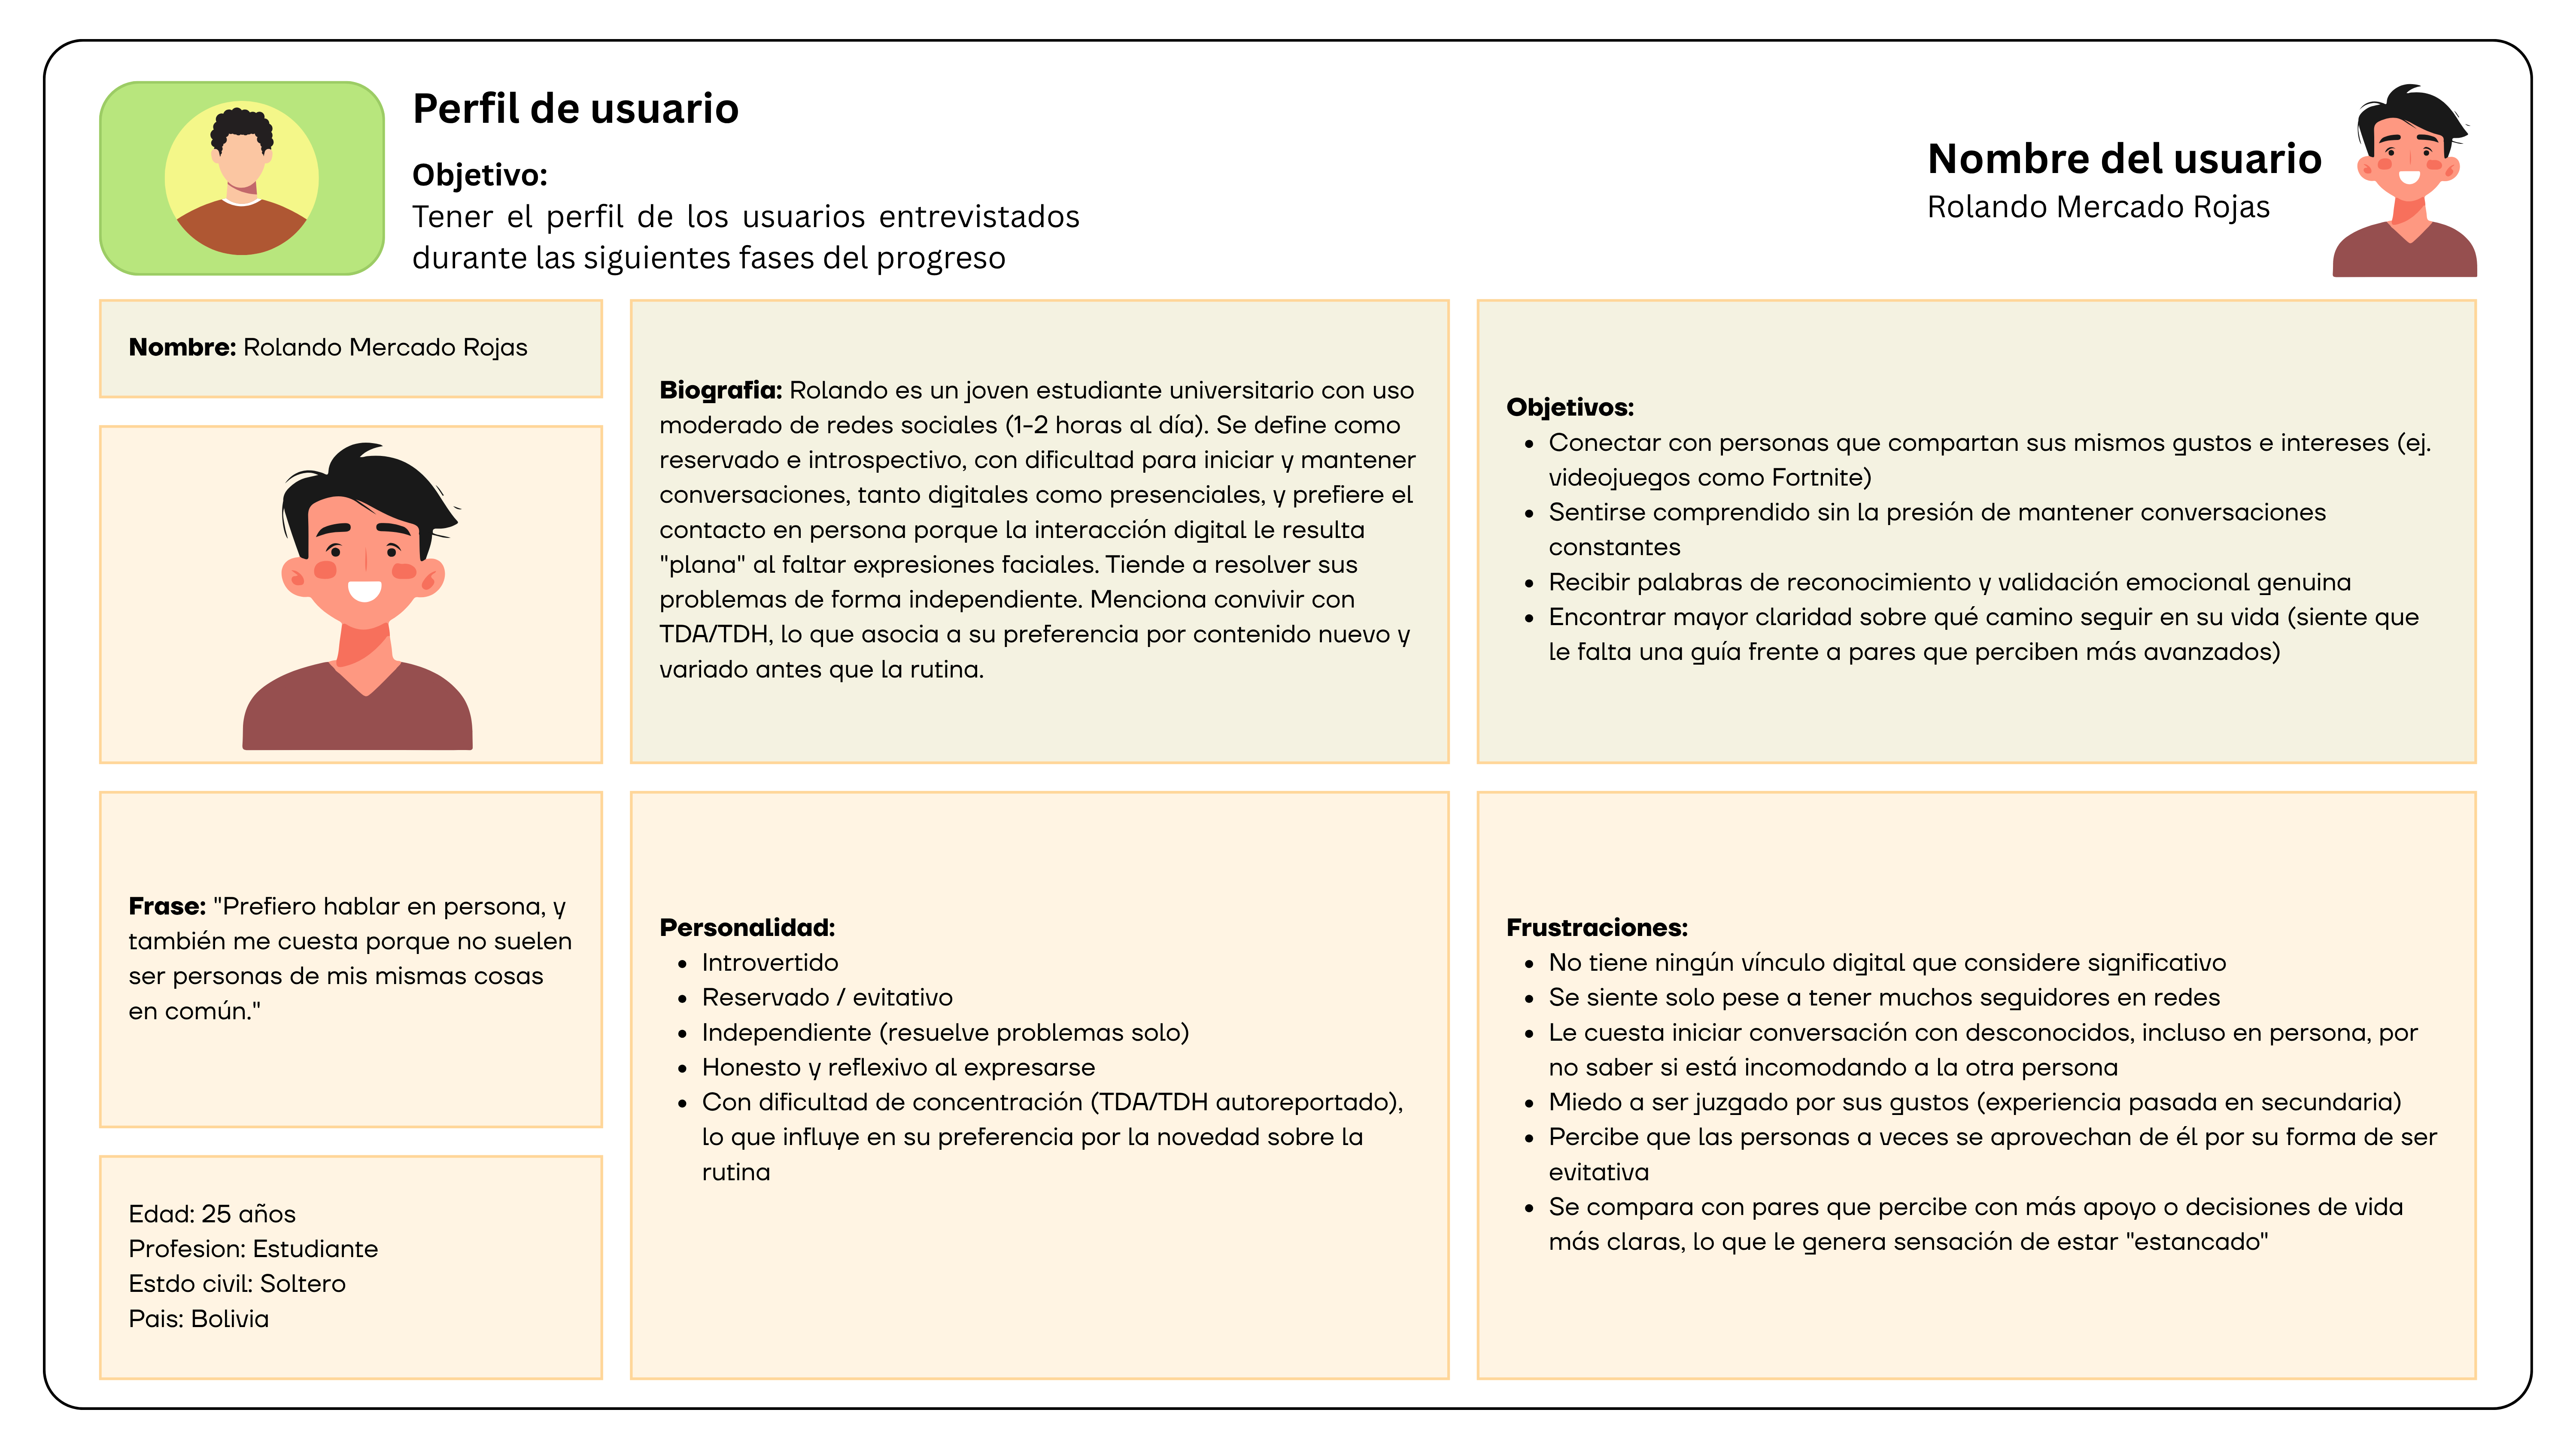
\includegraphics[width=0.9\textwidth]{Images/methodology/define/usuario1P.png}
  \vspace{4pt}
\end{figure}
\begin{center}
\small Fuente: Elaboración propia
\end{center}

El perfil de Rolando ilustra un patrón de aislamiento emocional pese a la conectividad digital, consistente con la discrepancia entre relaciones deseadas y disponibles descrita por Hawkley y Cacioppo (2010). Su frustración central, no tener ningún vínculo digital que considere significativo, sintetiza de forma individual la paradoja documentada a nivel poblacional por Feng et al. (2026).

\subsection{Usuario 5: Alejandra Pérez Ramal}
\begin{figure}[htbp]
  \centering
  \caption{Perfil de usuario - Usuario 5 (Alejandra Pérez Ramal)}
  \label{fig:perfil_usuario5}
  \vspace{4pt}
  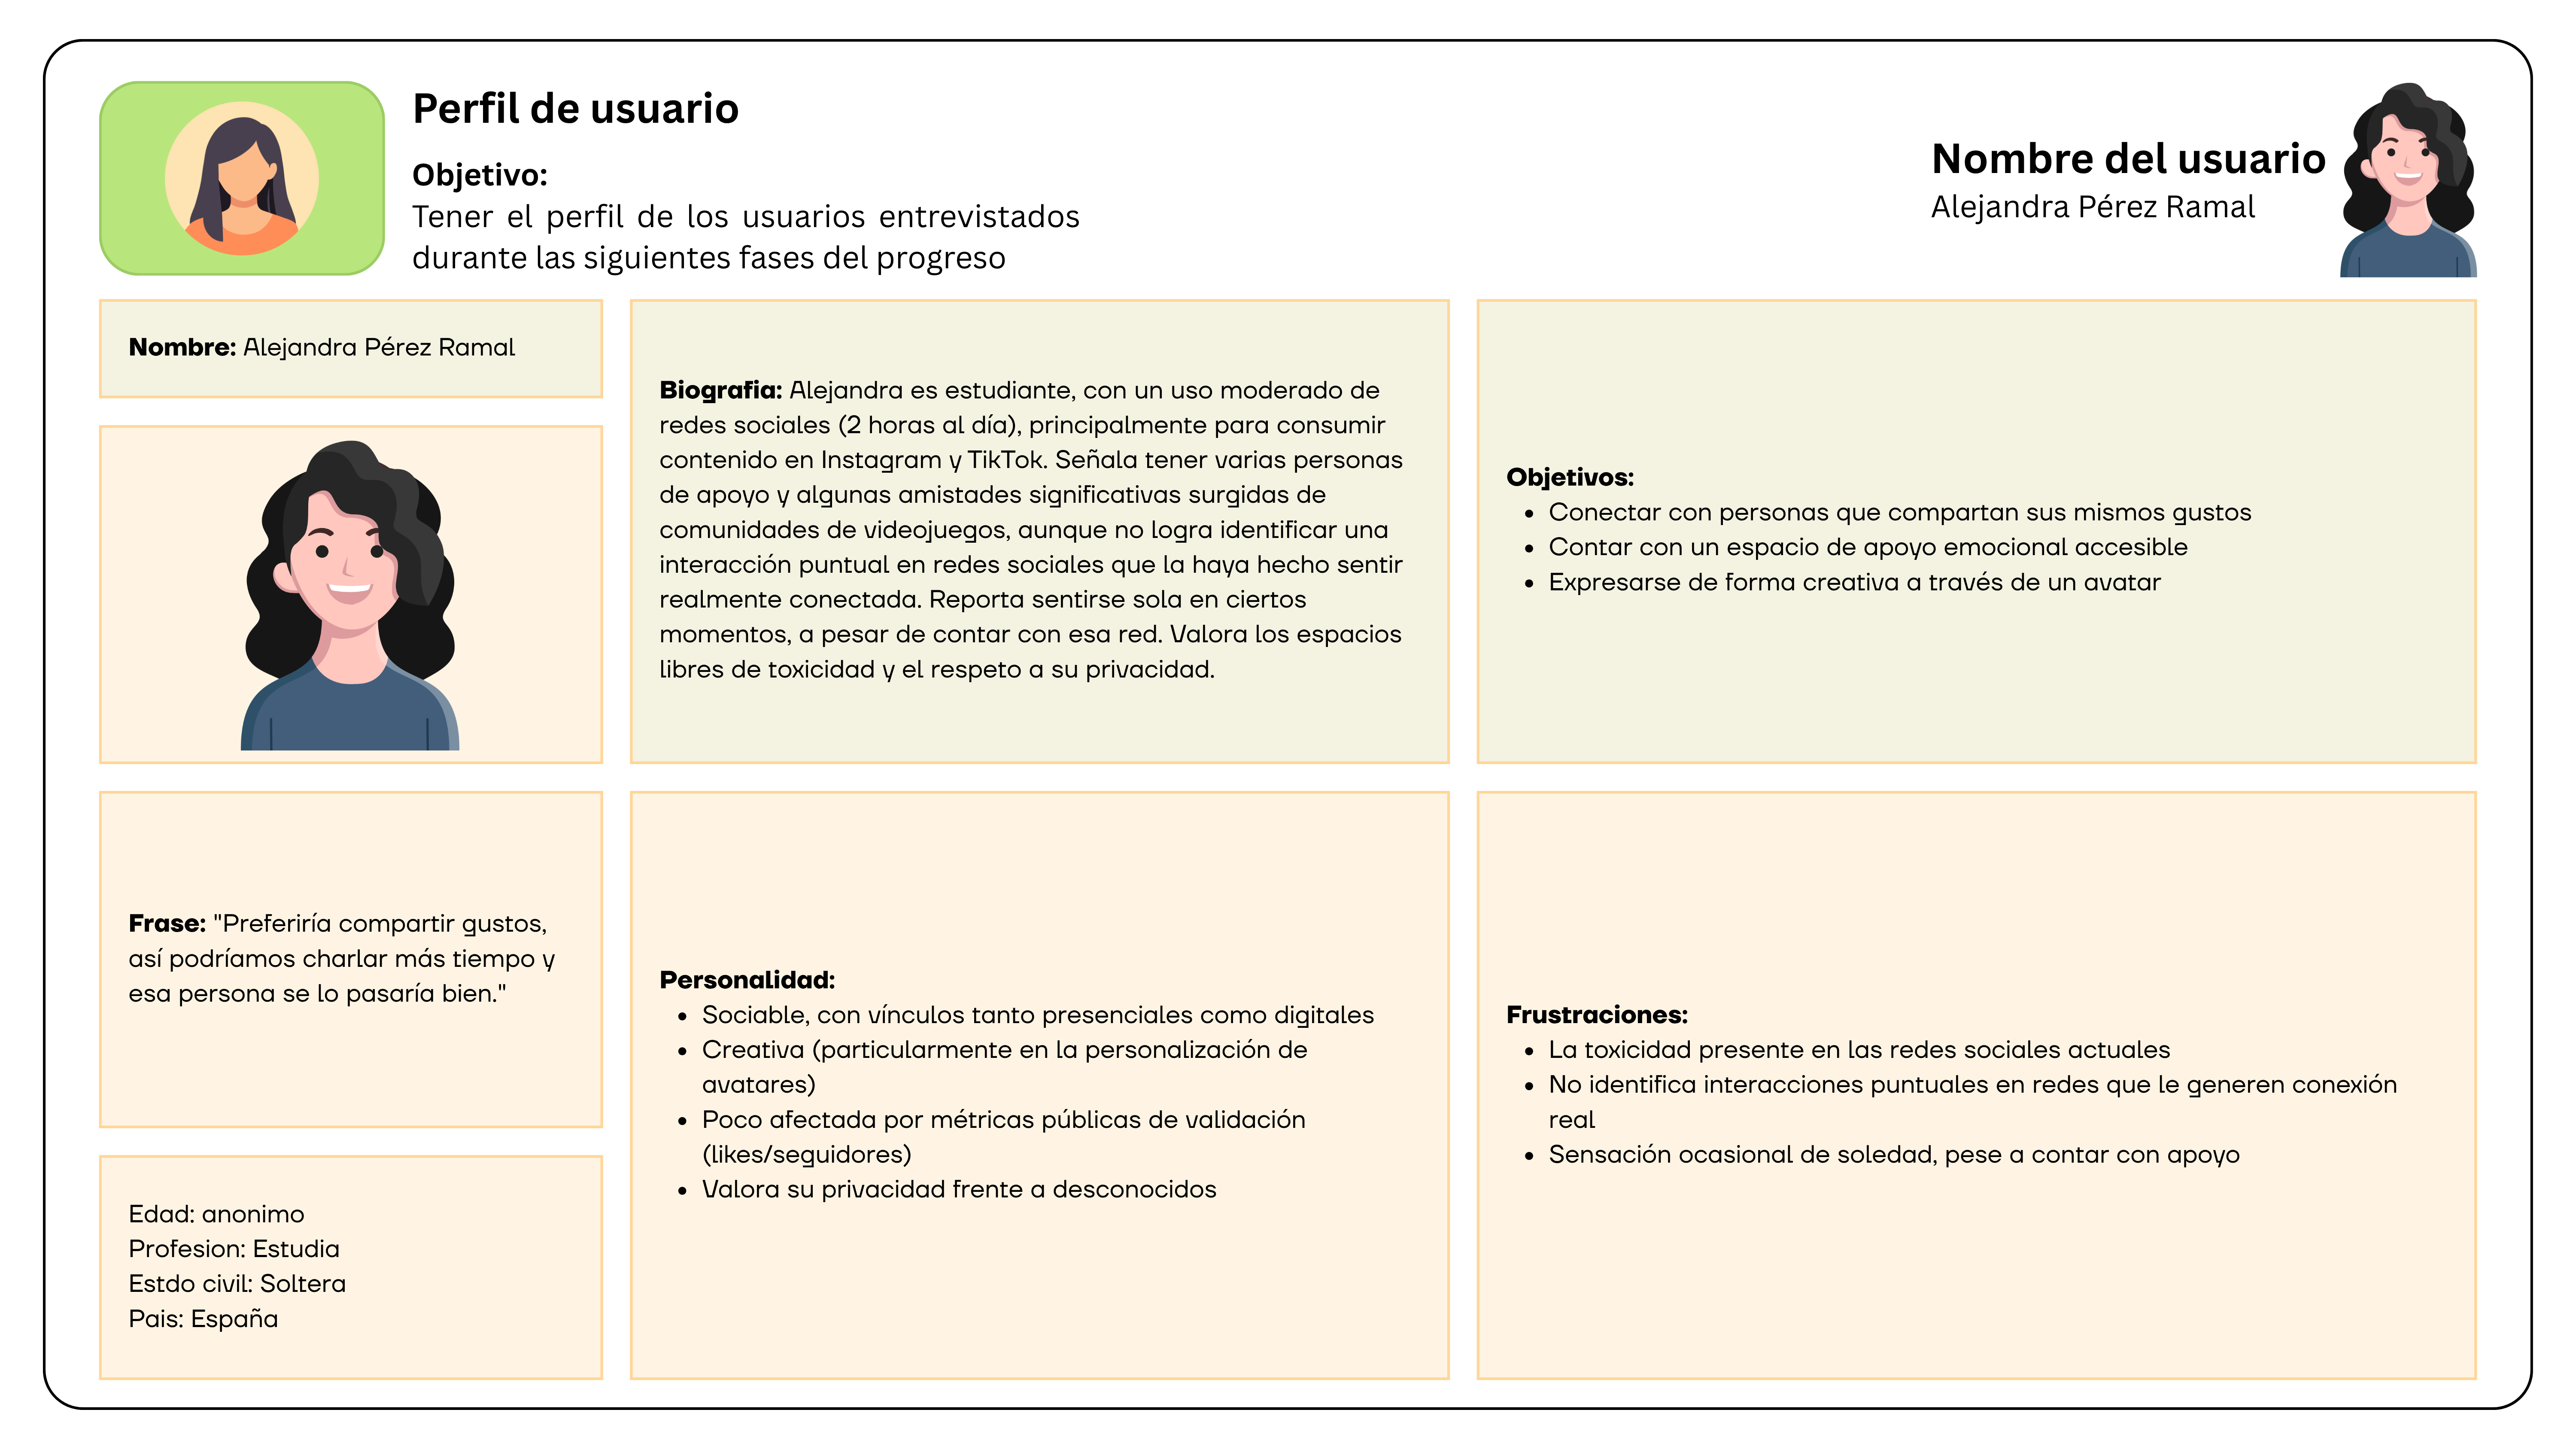
\includegraphics[width=0.9\textwidth]{Images/methodology/define/usuario5P.png}
  \vspace{4pt}
\end{figure}
\begin{center}
\small Fuente: Elaboración propia
\end{center}

El perfil de Alejandra aporta un matiz relevante al planteamiento del problema: a diferencia de Rolando, cuenta con vínculos significativos previos, surgidos de comunidades de videojuegos, lo que valida empíricamente el emparejamiento por intereses compartidos como mecanismo efectivo de vinculación (Liu et al., 2026). Sin perjuicio de ello, su experiencia de cautela relacional evidencia que la calidad del vínculo depende también de la gestión emocional de la interacción, y no únicamente de la afinidad temática.

\subsection{Usuarios 2, 3, 4 y 6}
De manera complementaria, se elaboraron los perfiles de los Usuarios 2 (Rubén Hernández Torrez), 3 (Fernando José Pérez Armando), 4 (Antonia Tapia) y 6 (Renata Martínez Mitte), cuyos perfiles refuerzan los hallazgos ya descritos: predominio del consumo pasivo, escasez de vínculos digitales significativos, y una valoración compartida hacia mecanismos de emparejamiento por afinidad y personalización mediante avatares.

\section{MAPA DE EMPATÍA}
Con el objetivo de sistematizar visualmente lo que cada usuario piensa, siente, escucha, ve, habla y hace, así como sus dolores y necesidades, se elaboró un Mapa de Empatía por participante, a partir de la información recogida en las entrevistas.

\subsection{Usuario 1: Rolando Mercado Rojas}
\begin{figure}[htbp]
  \centering
  \caption{Mapa de empatía - Usuario 1 (Rolando Mercado Rojas)}
  \label{fig:mapa_empatia_usuario1}
  \vspace{4pt}
  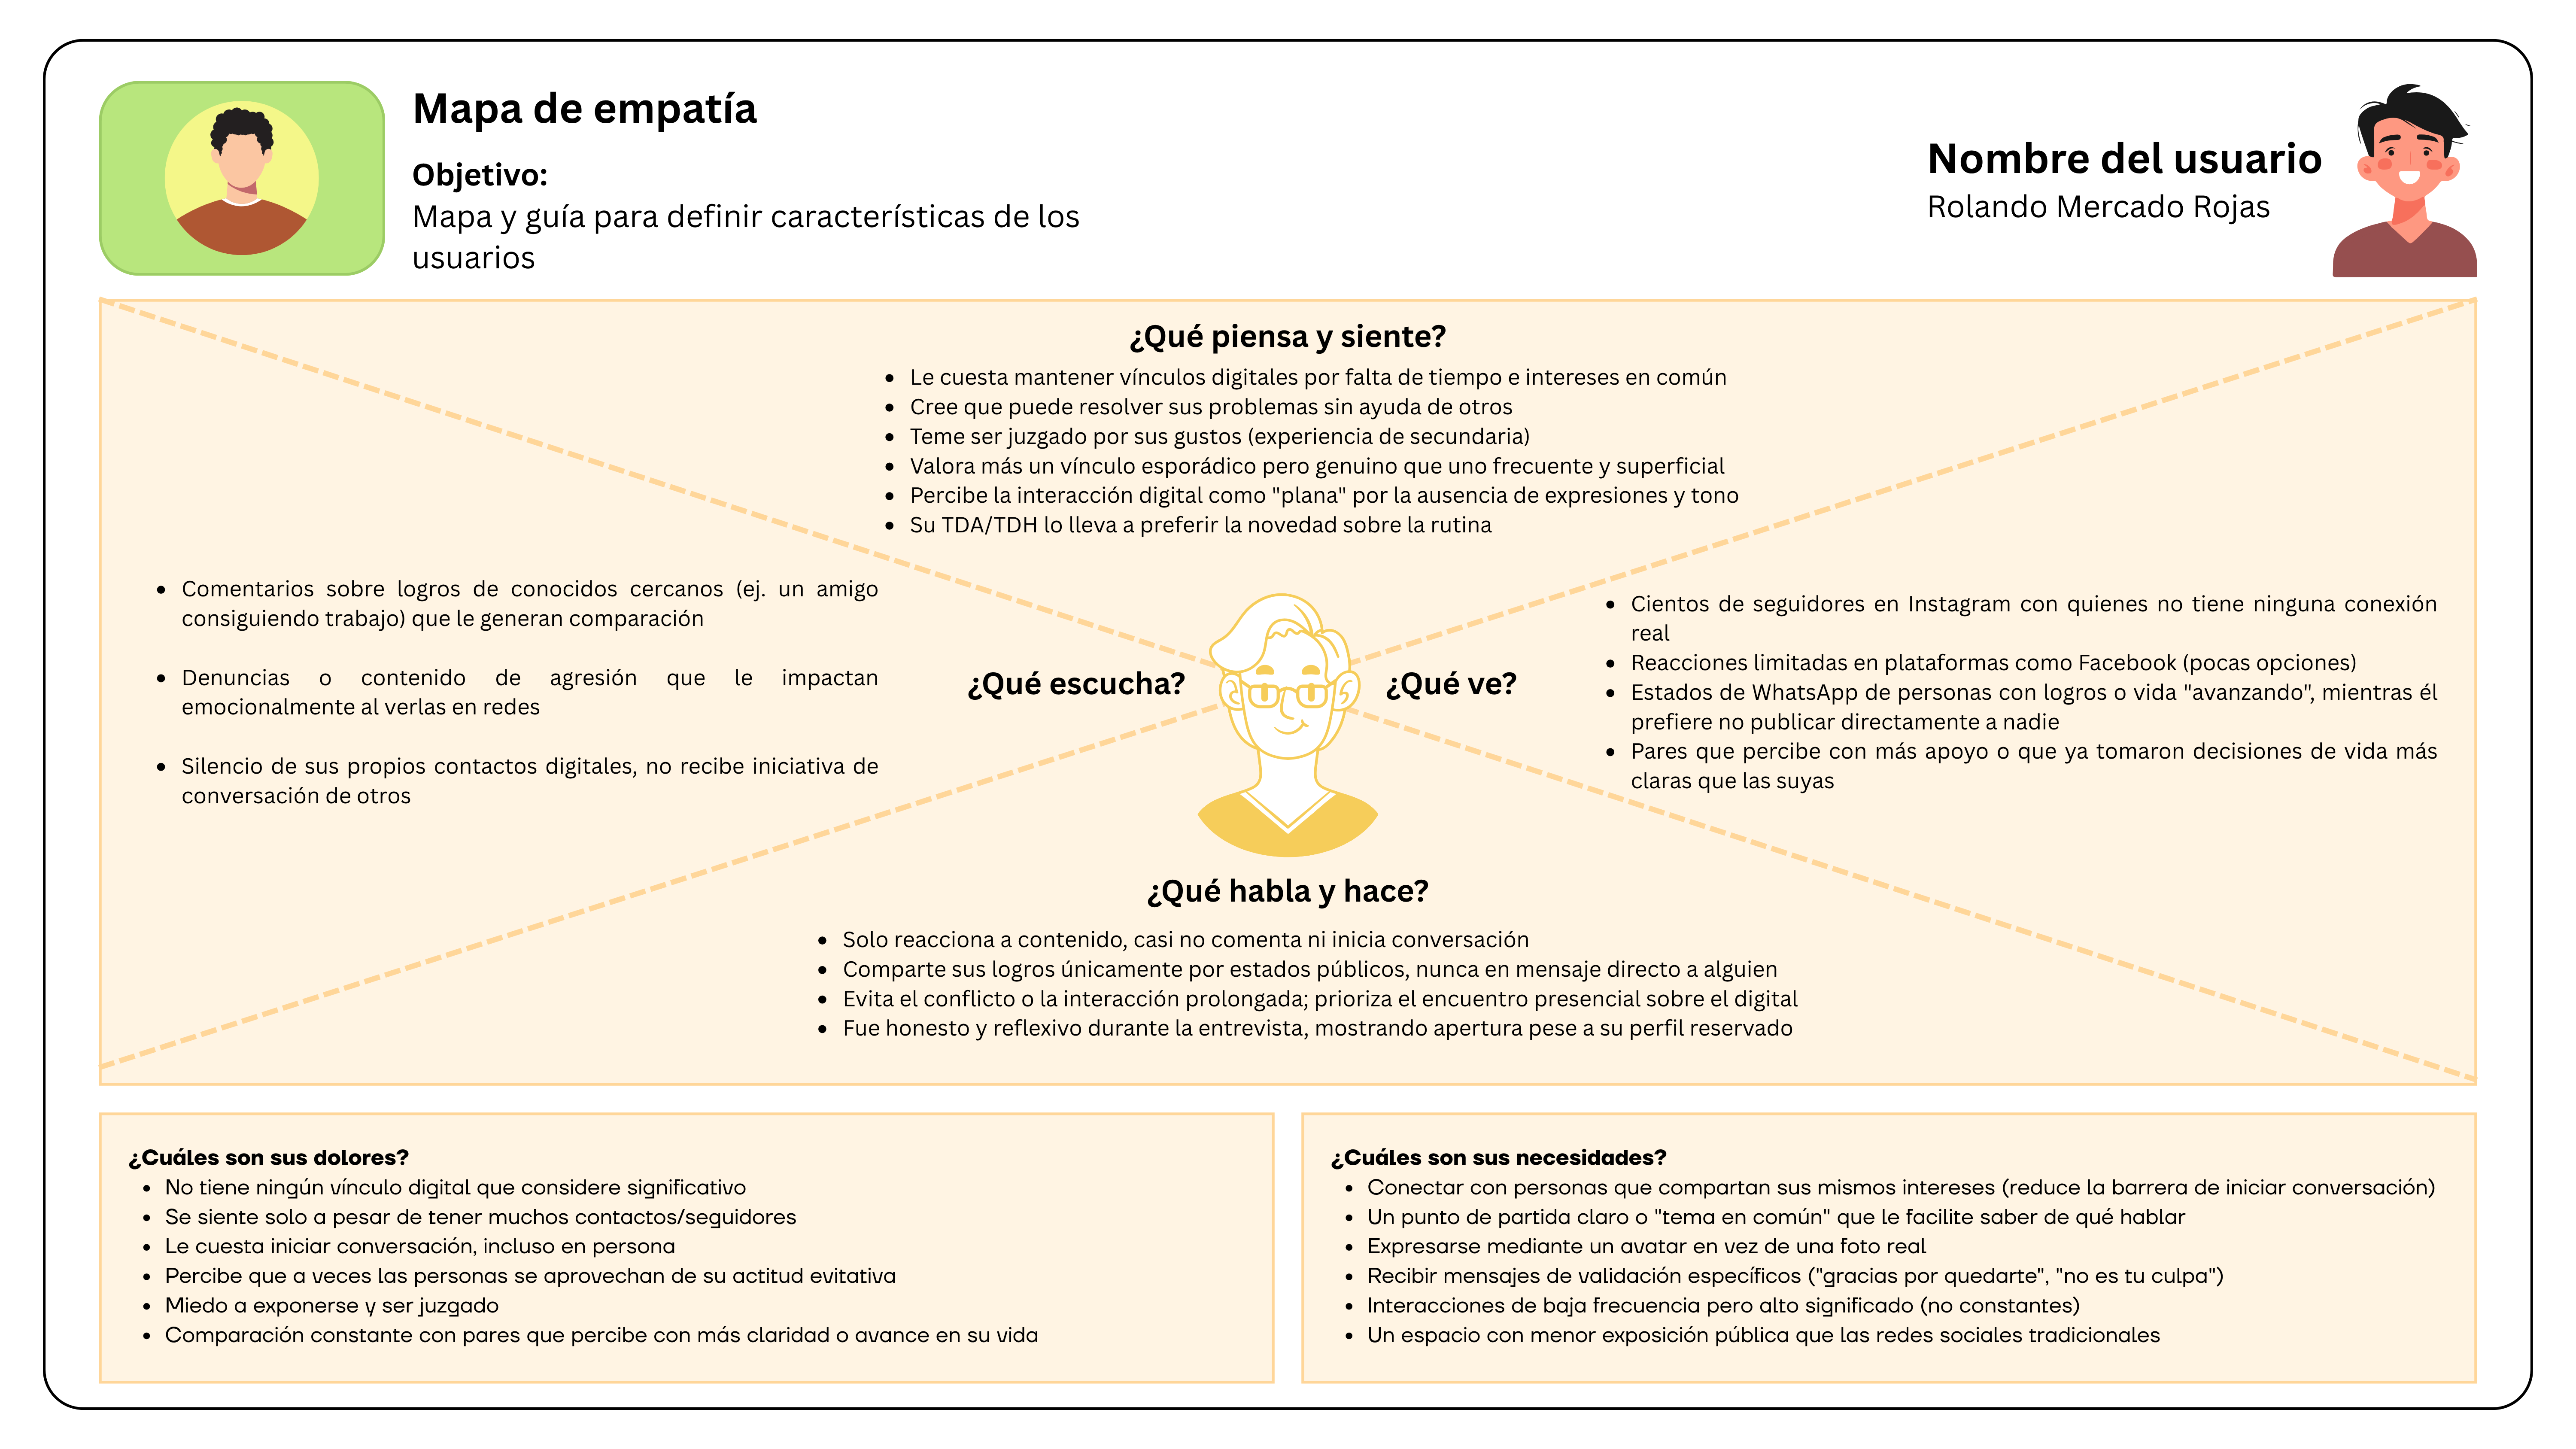
\includegraphics[width=0.9\textwidth]{Images/methodology/define/usuario1ME.png}
  \vspace{4pt}
\end{figure}
\begin{center}
\small Fuente: Elaboración propia
\end{center}

El mapa evidencia que la percepción de la comunicación digital como "plana", debido a la ausencia de expresiones y tono de voz, constituye un dolor central para Rolando, confirmando la advertencia de Picard (1997) sobre el empobrecimiento del canal emocional en la comunicación mediada por texto.

\subsection{Usuario 5: Alejandra Pérez Ramal}
\begin{figure}[htbp]
  \centering
  \caption{Mapa de empatía - Usuario 5 (Alejandra Pérez Ramal)}
  \label{fig:mapa_empatia_usuario5}
  \vspace{4pt}
  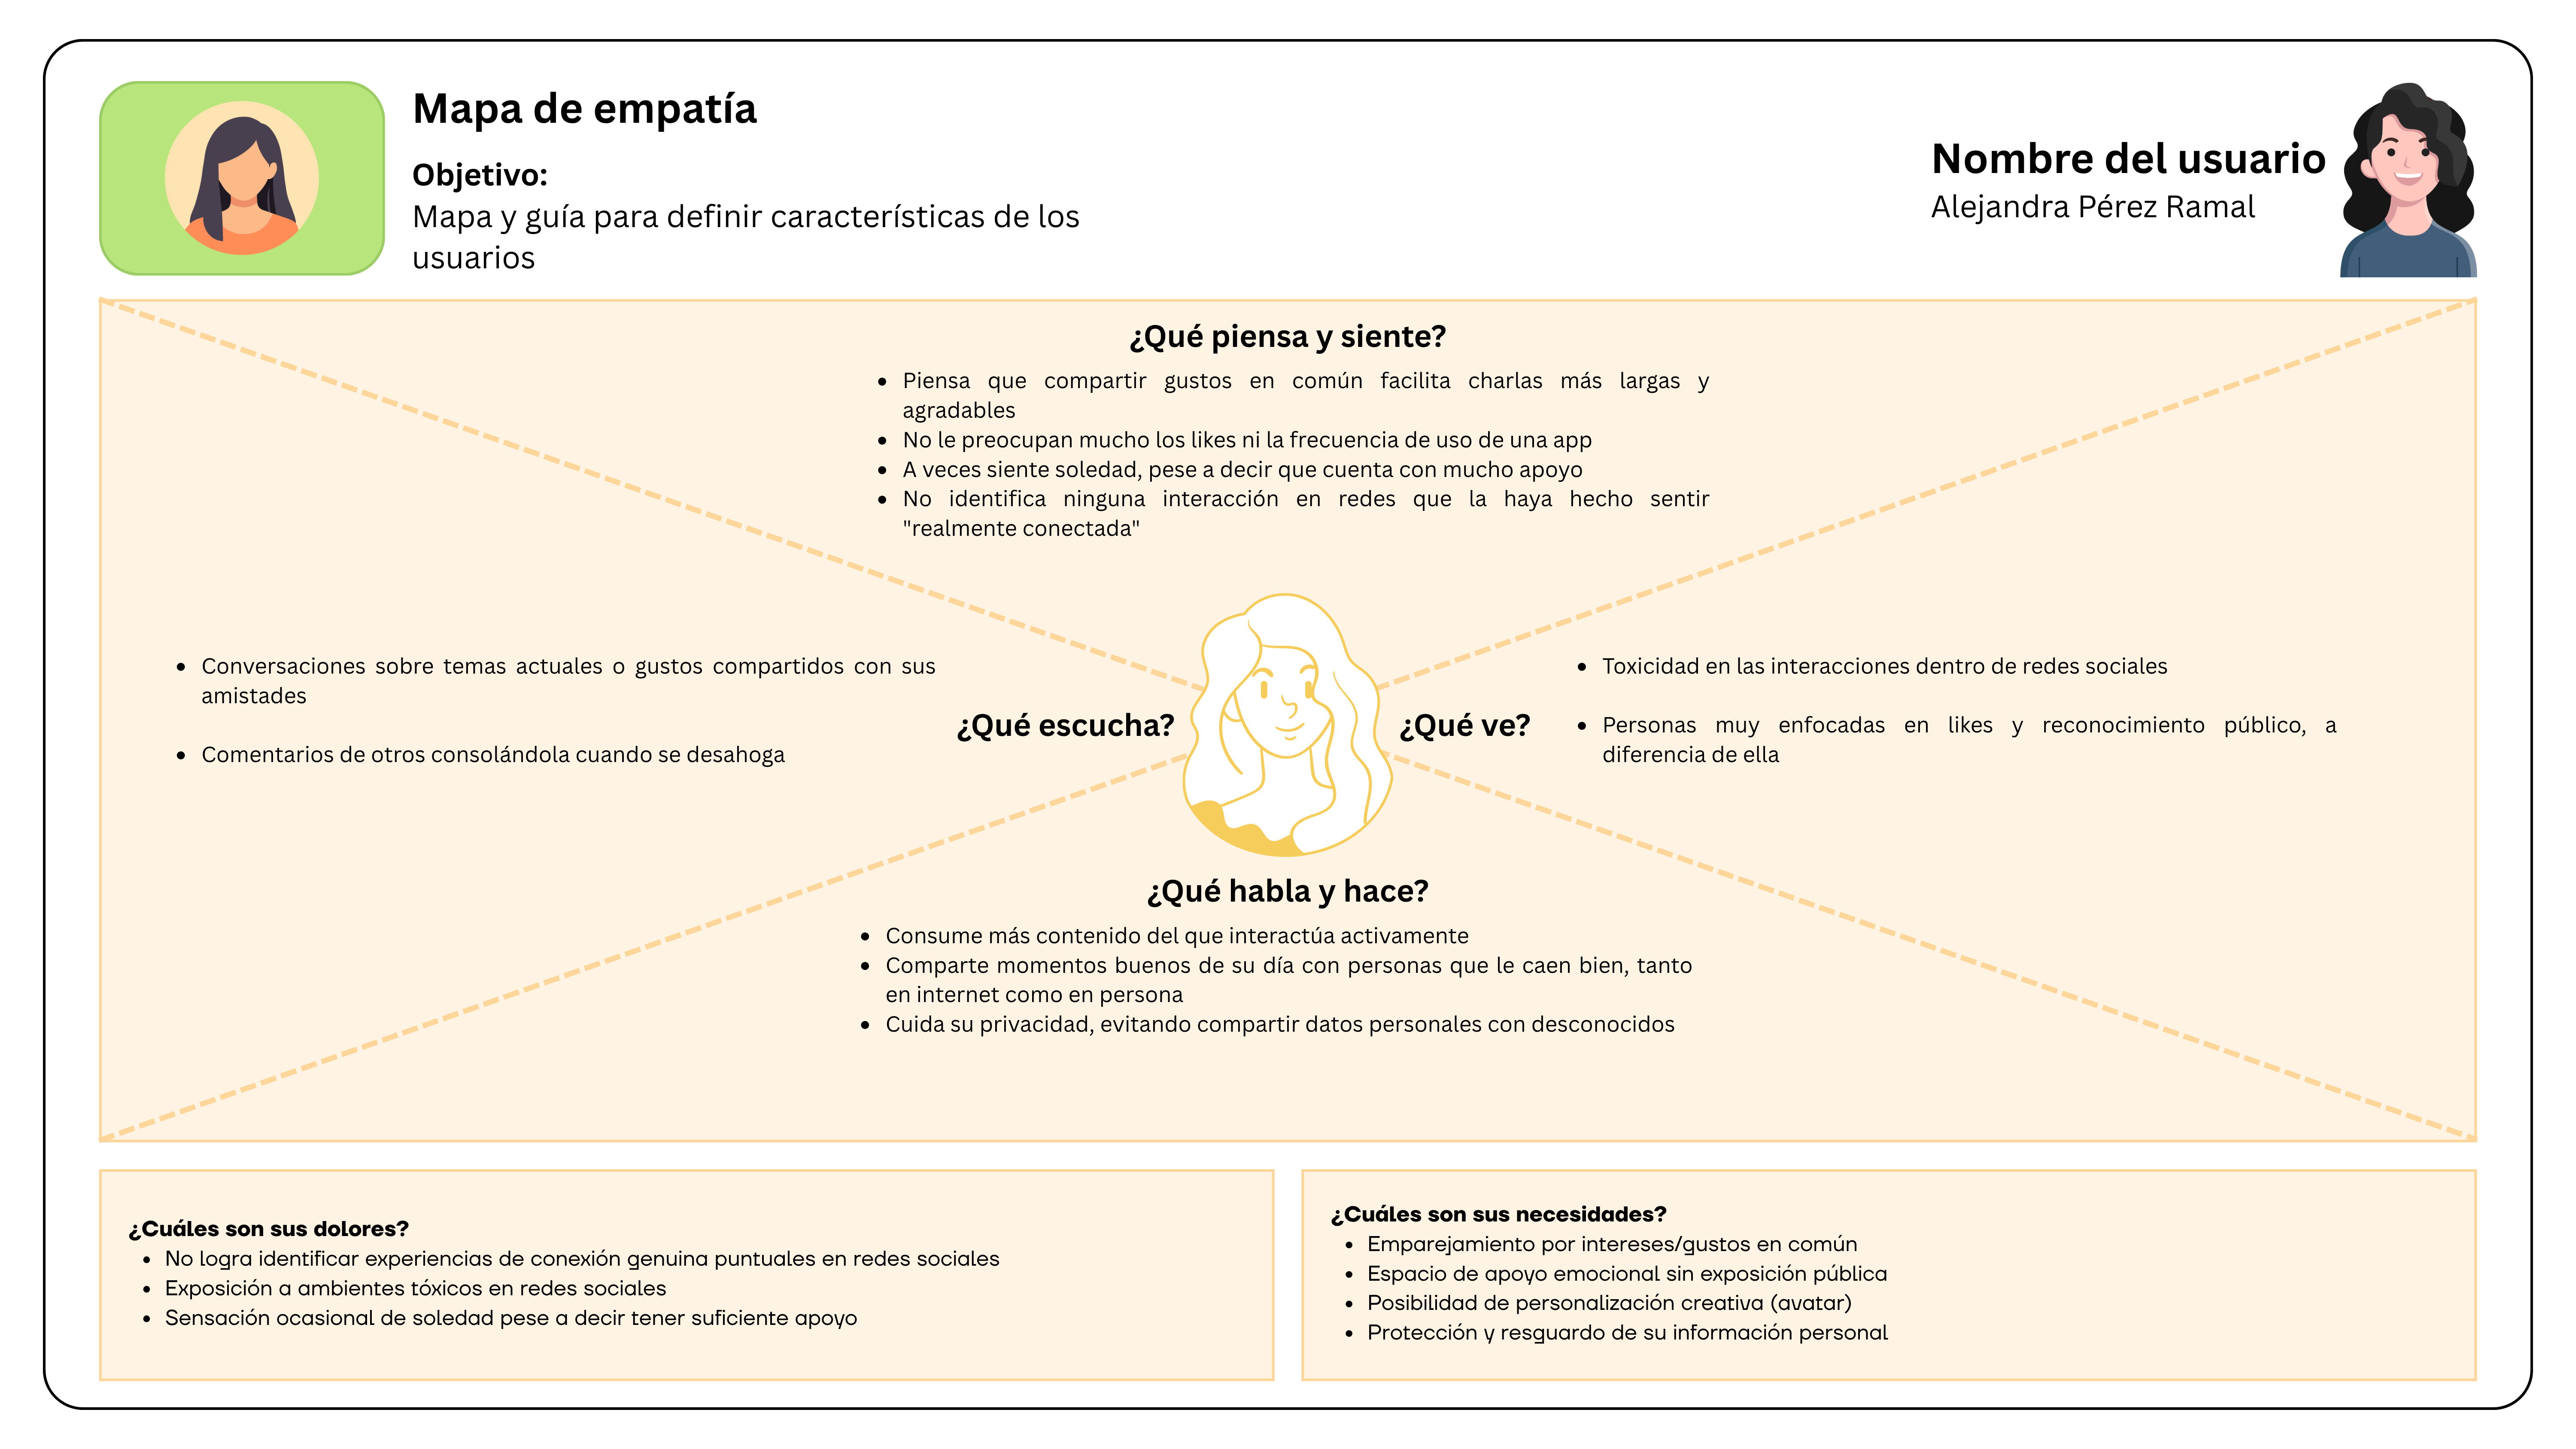
\includegraphics[width=0.9\textwidth]{Images/methodology/define/usuario5ME.png}
  \vspace{4pt}
\end{figure}
\begin{center}
\small Fuente: Elaboración propia
\end{center}

En el caso de Alejandra, el mapa revela una necesidad de protección de la privacidad frente a desconocidos como condición previa para la confianza, lo que resulta coherente con los mecanismos de seguridad y moderación contemplados en el alcance del proyecto.

\subsection{Usuarios 2, 3, 4 y 6}
Los Mapas de Empatía correspondientes a los Usuarios 2 (Rubén Hernández Torrez), 3 (Fernando José Pérez Armando), 4 (Antonia Tapia) y 6 (Renata Martínez Mitte) confirman de forma reiterada los mismos dolores y necesidades: escasos vínculos digitales significativos, exposición a ambientes hostiles o de comparación social, y una necesidad compartida de espacios que prioricen la calidad de la interacción sobre la exposición pública.

\section{MAPA DE MOTIVACIONES}
Con el objetivo de identificar variables positivas compartidas entre los distintos usuarios respecto a sus necesidades, se elaboró un Mapa de Motivaciones cruzando la información de los seis participantes entrevistados.

\begin{figure}[htbp]
  \centering
  \caption{Mapa de motivaciones}
  \label{fig:mapa_motivaciones}
  \vspace{4pt}
  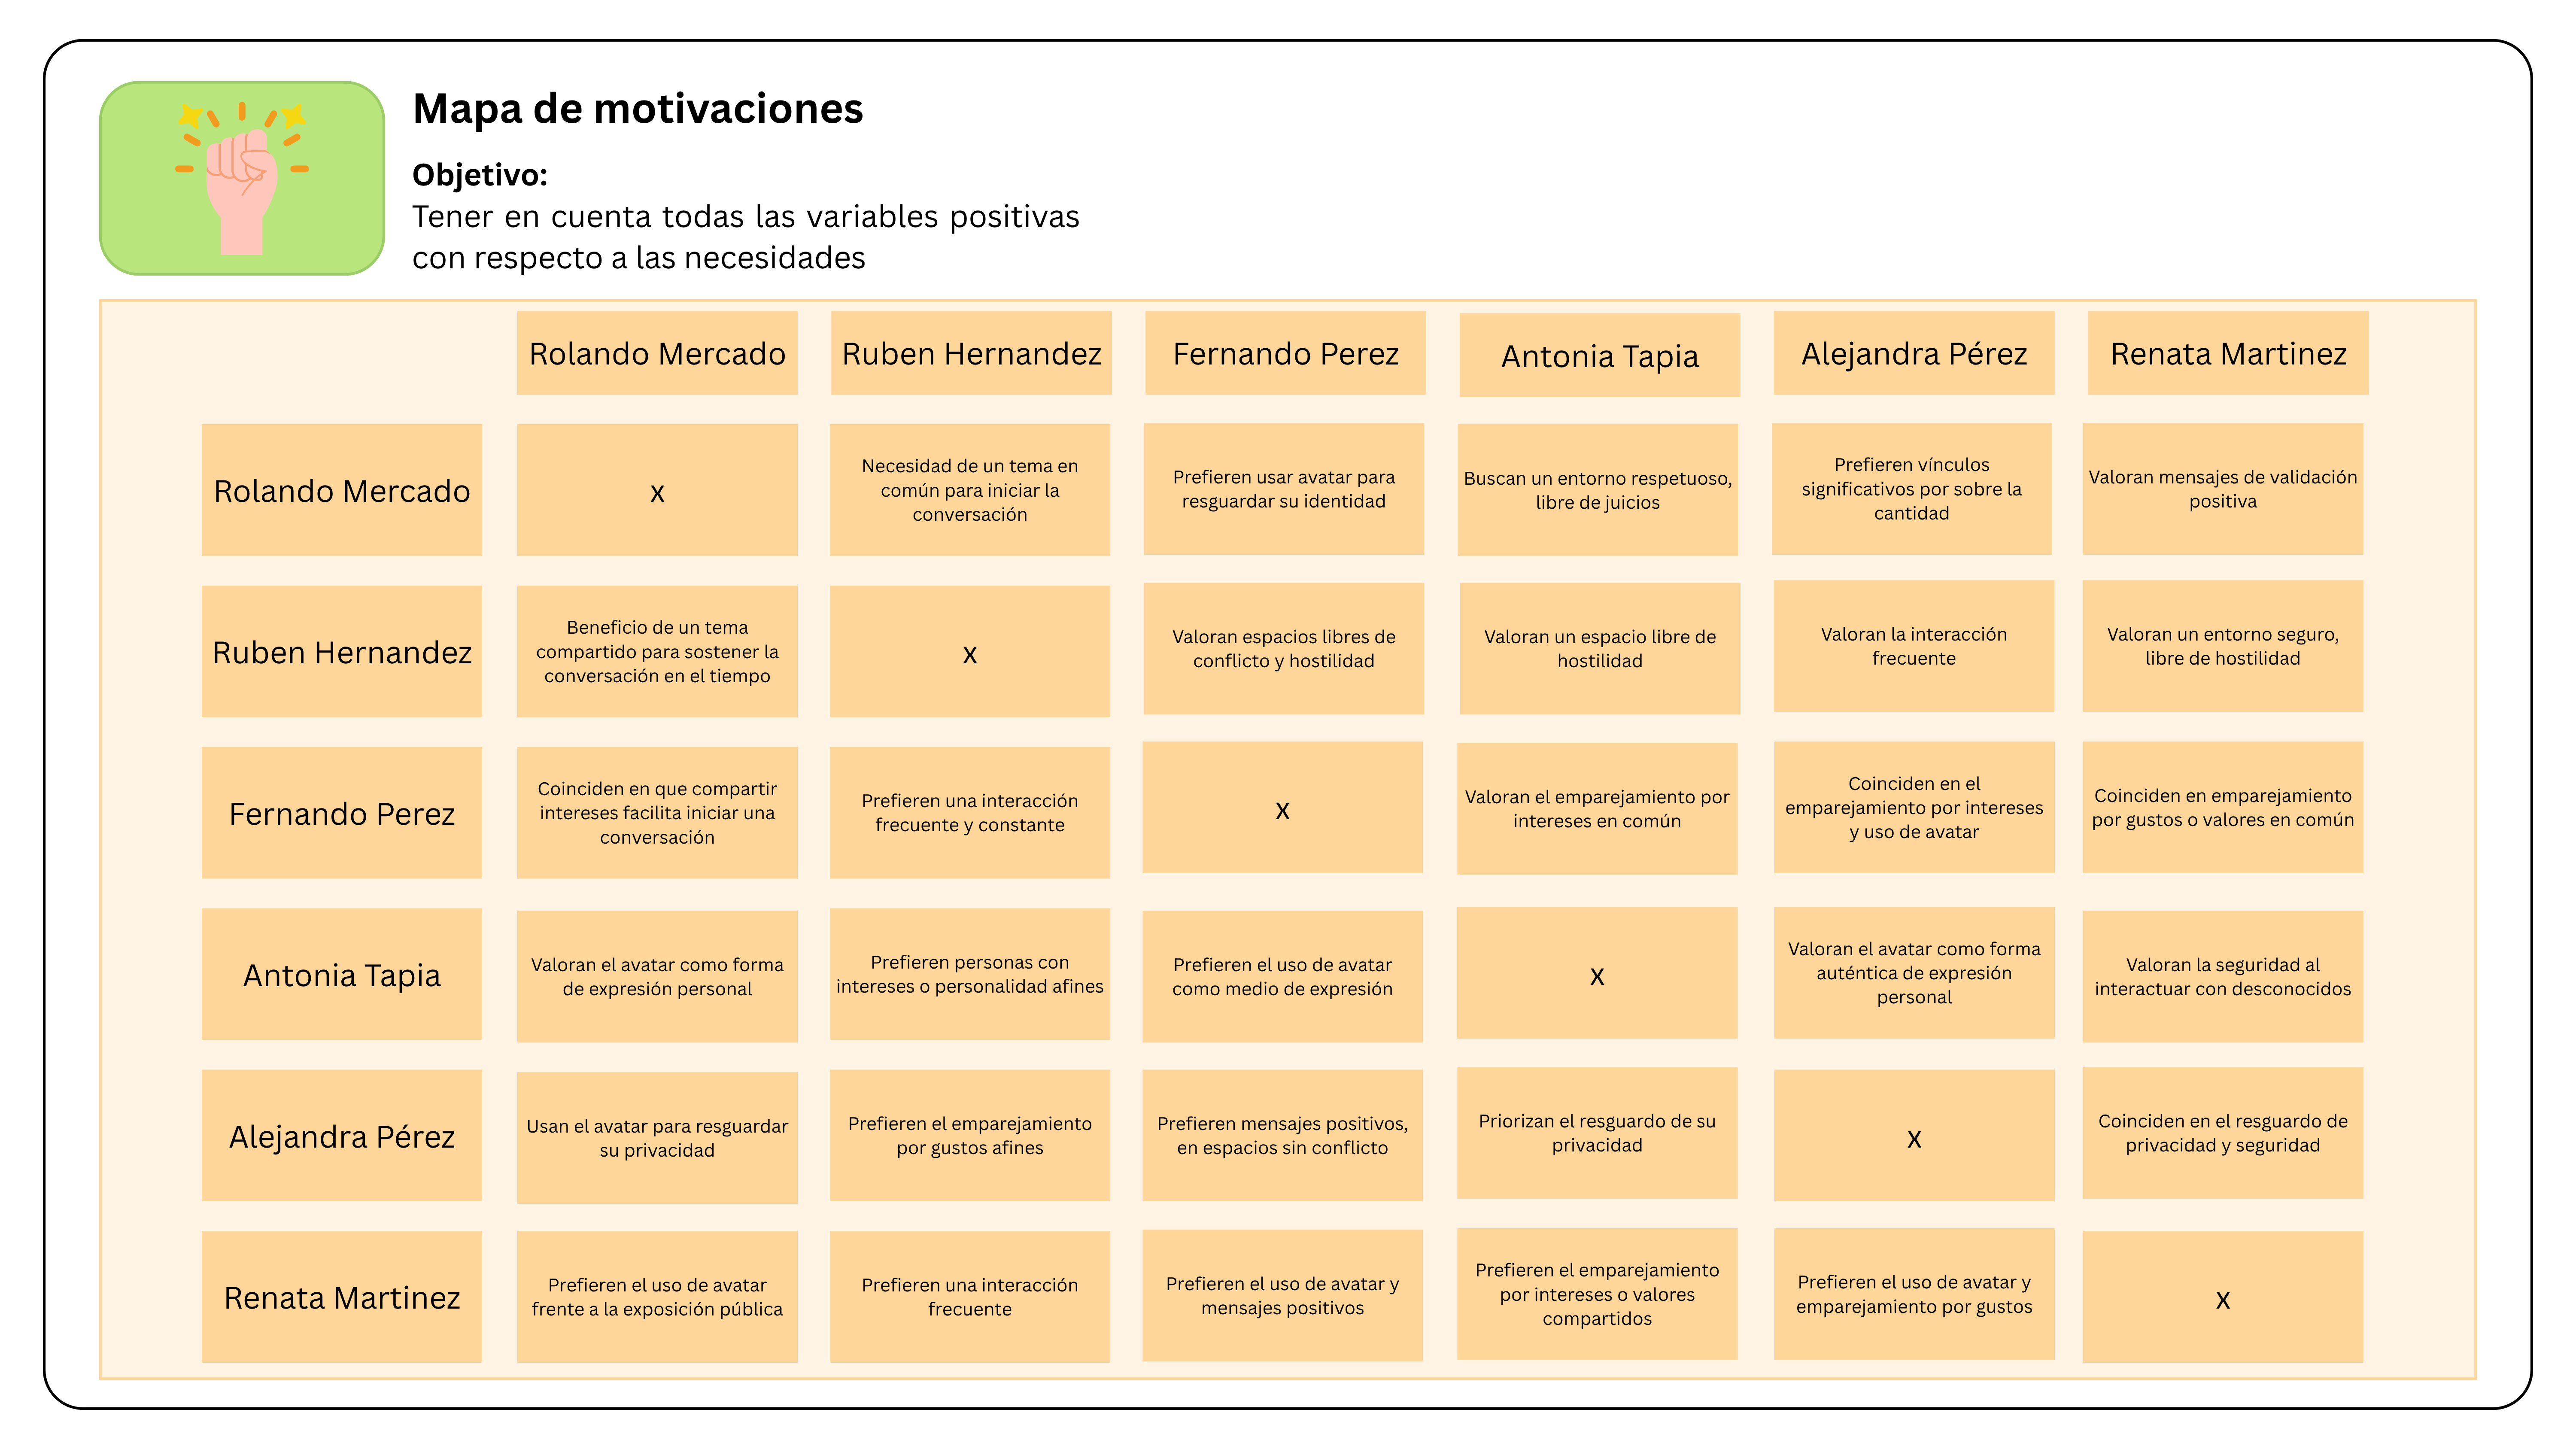
\includegraphics[width=0.95\textwidth]{Images/methodology/define/mapaDeMotivaciones.png}
  \vspace{4pt}
\end{figure}
\begin{center}
\small Fuente: Elaboración propia
\end{center}

El análisis cruzado permitió identificar tres motivaciones que se repiten de manera consistente entre la mayoría de los participantes: (a) la necesidad de un interés o gusto en común como facilitador de la conversación, presente en 13 de los 15 cruces analizados; (b) la preferencia por el uso de un avatar como medio de expresión y resguardo de la identidad, presente en 12 de los 15 cruces; y (c) la necesidad de un entorno libre de hostilidad o conflicto, presente en 6 de los 15 cruces. Estos hallazgos, obtenidos de forma inductiva a partir de la evidencia primaria, coinciden con los factores identificados deductivamente a partir de la literatura en el Capítulo 3, en particular con los planteamientos de Godard y Holtzman (2024) sobre el valor del uso activo y recíproco, y con el modelo de vinculación social propuesto por Takano (2018).

\section{¿CÓMO PODRÍAMOS...?}
A partir de los conocimientos sintetizados en el Mapa de Motivaciones, se aplicó la técnica ¿Cómo podríamos...? con el objetivo de convertir dichos hallazgos (insights) en preguntas orientadoras que faciliten la posterior generación de ideas en la etapa de Idear.

\begin{figure}[htbp]
  \centering
  \caption{Técnica ¿Cómo podríamos...?}
  \label{fig:como_podriamos}
  \vspace{4pt}
  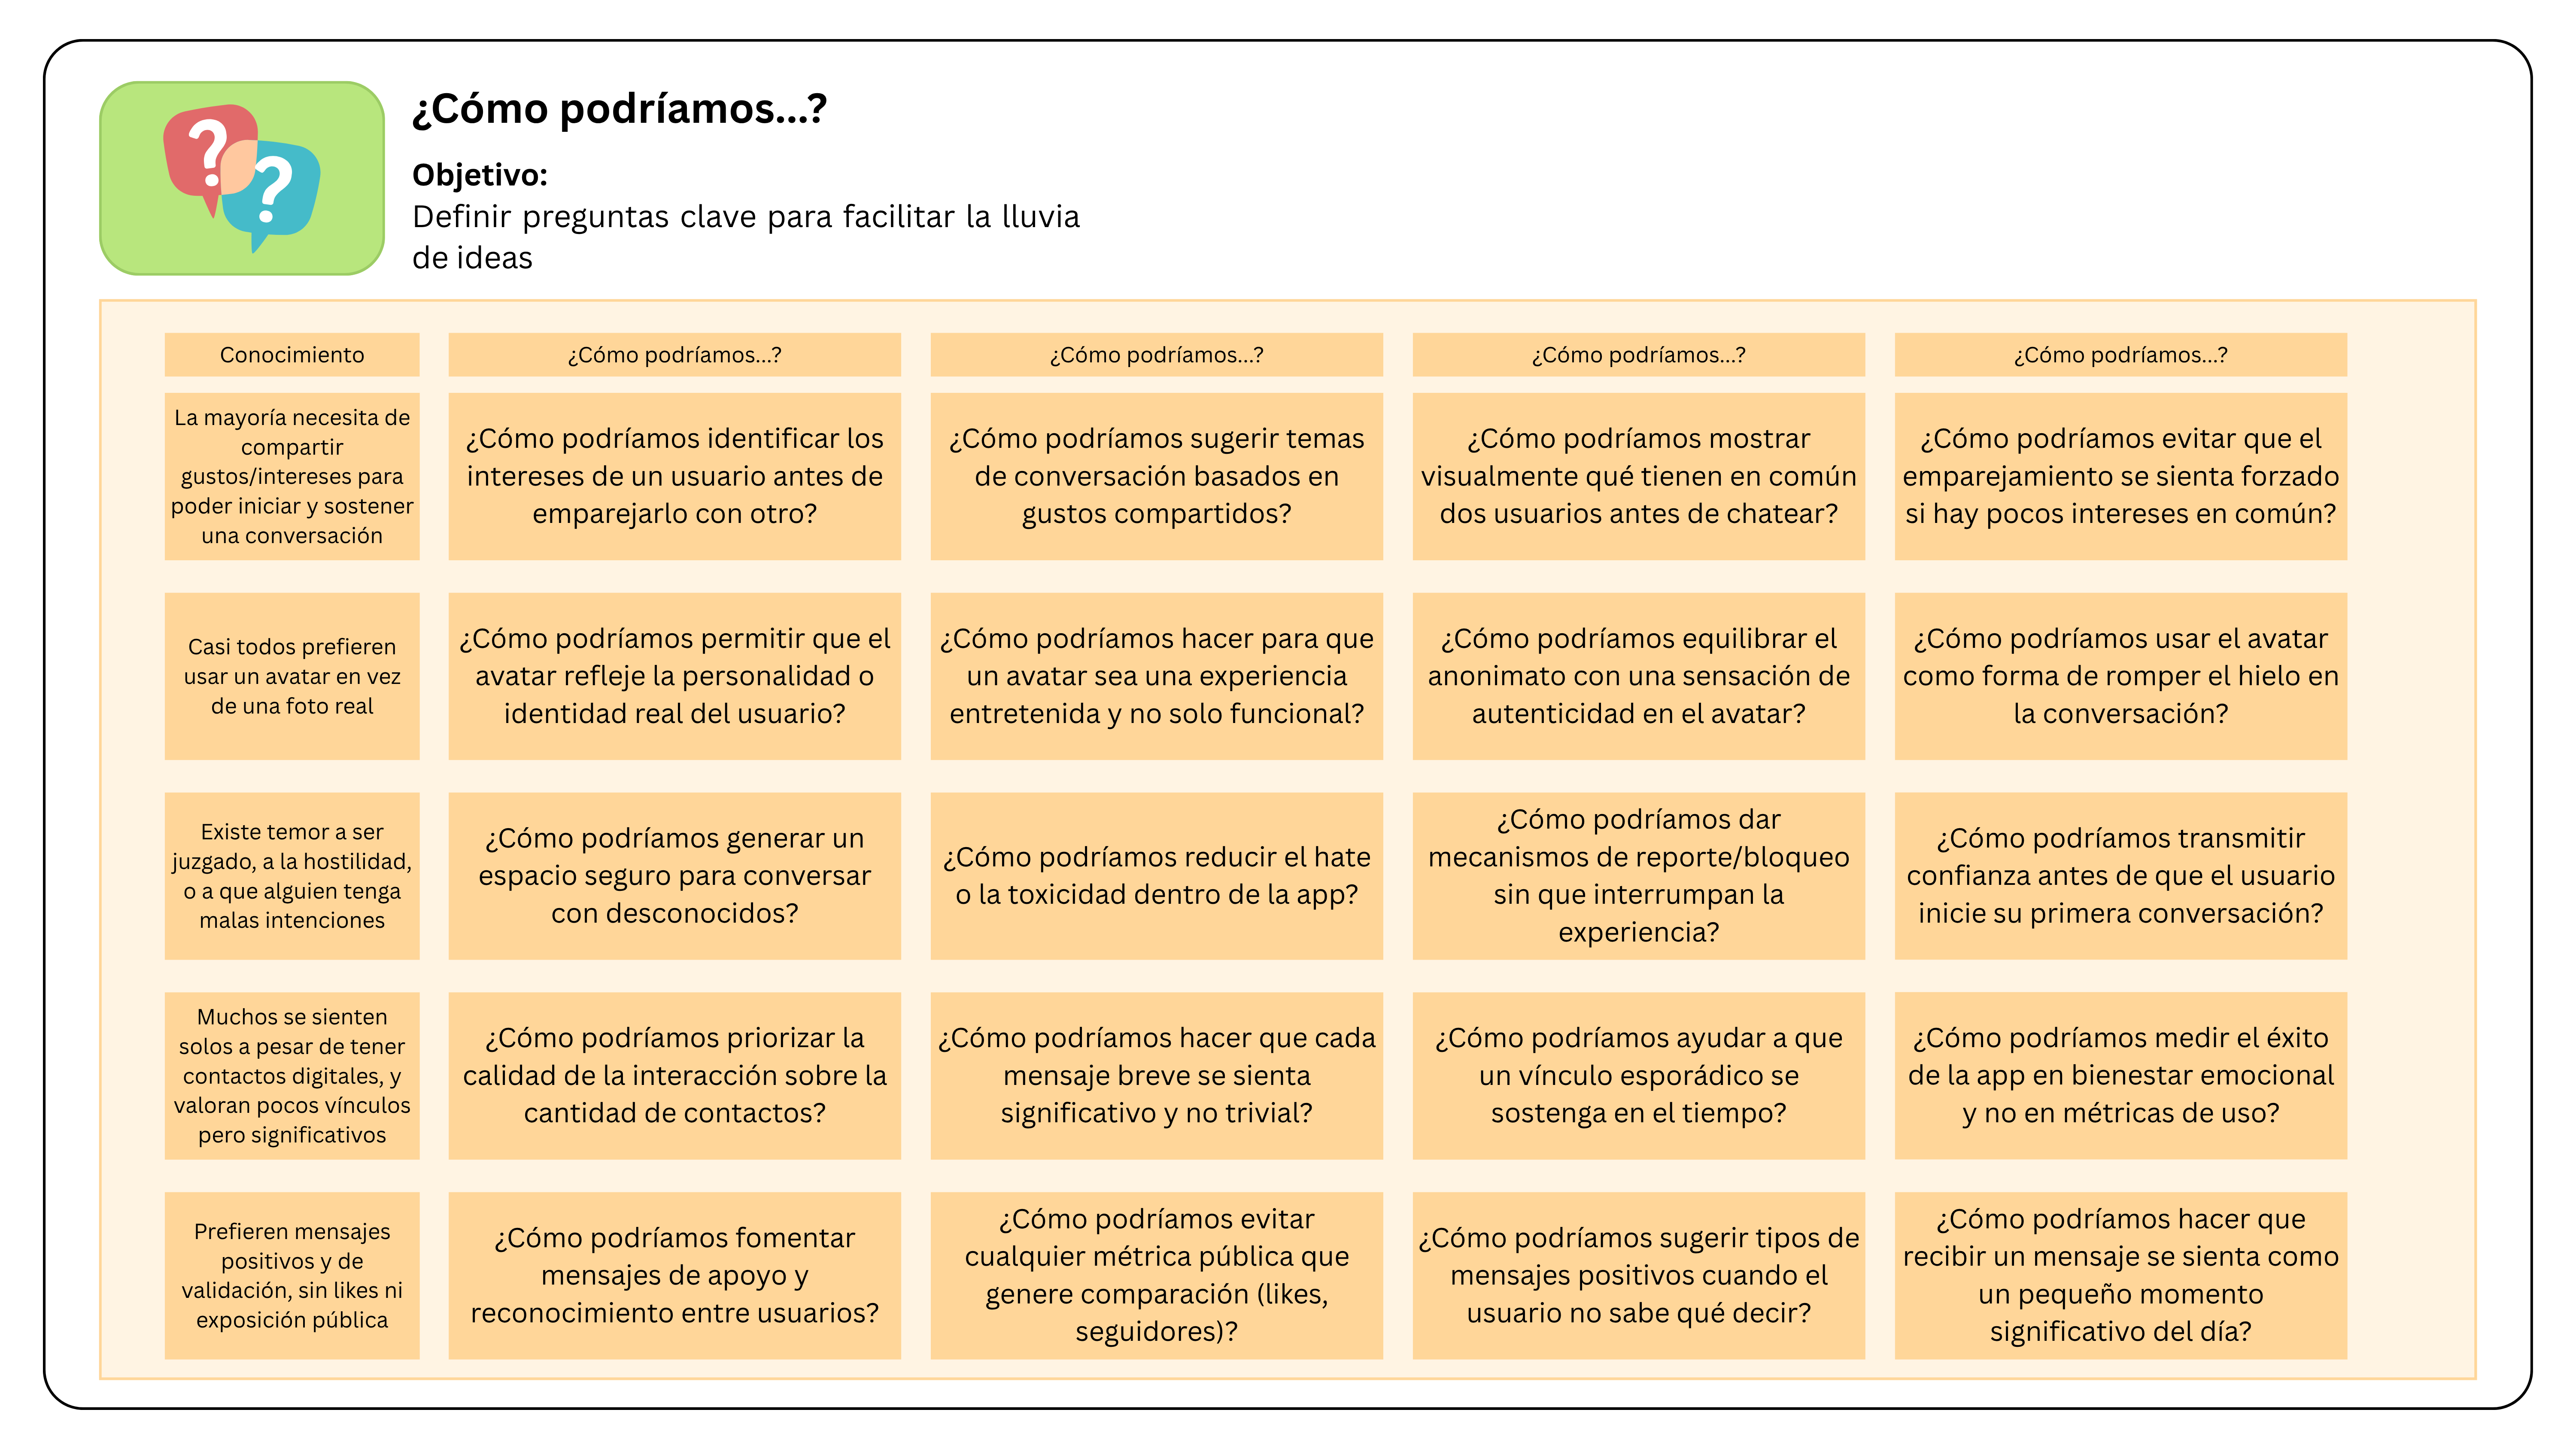
\includegraphics[width=0.95\textwidth]{Images/methodology/define/comoPodriamos.png}
  \vspace{4pt}
\end{figure}
\begin{center}
\small Fuente: Elaboración propia
\end{center}

Las preguntas formuladas abordan los cinco conocimientos centrales derivados de la fase de Empatizar: la necesidad de intereses compartidos, la preferencia por el uso de avatares, el temor a la hostilidad o a interactuar con desconocidos, la preferencia por vínculos pocos pero significativos, y la preferencia por mensajes positivos libres de métricas públicas de validación. Estas preguntas constituyen el punto de partida directo para la generación de ideas desarrollada en el Capítulo 6.

\section{PLANTEAMIENTO DEL PROBLEMA (POINT OF VIEW)}
A partir de la síntesis de la evidencia documental (Capítulo 3) y de la evidencia primaria recolectada en el presente capítulo, se formula el siguiente planteamiento del problema (POV), en los términos propuestos por Vargas Márquez et al. (2021):

\begin{quote}
Los jóvenes de 16 a 28 años necesitan un espacio digital que priorice la calidad de la interacción sobre la cantidad de conexiones, porque las plataformas actuales, centradas en el consumo pasivo de contenido y en métricas públicas de validación, no logran satisfacer su necesidad de vínculos genuinos, generando una desconexión emocional pese a la hiperconectividad.
\end{quote}

Este planteamiento integra los hallazgos más consistentes de la fase de Empatizar —la necesidad de afinidad temática, la preferencia por el anonimato progresivo mediante avatares, la exigencia de seguridad frente a desconocidos y la preferencia por vínculos escasos pero significativos— y constituye la base sobre la cual se desarrollan las técnicas de generación de ideas en el Capítulo 6.